\chapter{Latent Variable Neural Machine Translation}

In this chapter we describe the \ac{LVNMT} models we considered as part of our analysis. We begin by describing the underlying \ac{NMT} architecture common to both approaches. We then describe our discriminative model $p(y \cond{x})$, and our generative model $p(x, y)$. The final section discusses the practical details of representing the latent variables and defining the inputs from the appropriate components in each architecture. Throughout this chapter, we will often reference vectors as $\mathbb{R}^{n}$ but the actual dimensions for these vectors does not mean all the vectors are of the same dimensions and will otherwise specify the actual dimension whenever appropriate. 


\section{Neural Architecture}

In this section we explain the base neural architecture which our \ac{LVNMT} build from. Inherently, there is nothing necessarily unique to this architecture for incorporating latent variables.  The ideas in each \ac{LVNMT} model considered are applicable to alternative neural architectures, such as the Transformer \cite{vaswani2017attentionTransformer}, which may benefit from introduced latent variables as well. 

The \ac{NMT} architecture we consider is a \ac{seq2seq} model proposed by the work of  \citet{bahdanau2014NMTBYJoint}. The core components include source \& target word embeddings, an encoder, attention mechanism, and decoder. We describe all the layers except the word embeddings which are projections of the vocabulary for each language into a continuous space $\mathbb{R}^{n}$. When we refer words $x_{i}$ or $y_{i}$, these actually correspond to each word's associated word embedding as inputs to the model.  

\subsection{Encoder}
The encoder is a bi-directional \ac{RNN} which generates hidden states from reading the source sequence $x$ both forwards and backwards. Formally, the \ac{RNN} produces forward hidden states $h^{f}_{i} \in \mathbb{R}^{n}$ for each input word $x_{i}$, where $h^{f}_{i}$ is conditioned on all previous $x_{<i}$ words through $h_{i-1}^{f}$, and previous word embedding. The sequence is then read backwards by the \ac{RNN} to produce hidden states $h^{b}_{i} \in \mathbb{R}^{n}$ for each word $x_{i}$ where each $h^{b}_{i}$ is conditioned on all subsequent words in the sentence $x_{>i}$. The final hidden states are a concatenation of these complementary embeddings $h_{i}  = [h^{f}_{i} ; h^{b}_{i}]$ $ \forall i \in [0,...,T]$ where $T$ is the sentence length. Intuitively, each $h_{i}$ can be viewed as a contextual embedding of each source word in the sentence. These embeddings are utilized in the decoder via the \textit{Global Attention} mechanism, described next. %This information improves the translation quality beyond initializing the decoder through the attention mechanism, described next. 

\subsection{Global Attention}

Global attention mechanisms, in the context of \ac{seq2seq} models, generally refer to combining information from all the encoder hidden states to inform the decoding process. This is achieved by a function of the current decoder state $s_{j}$ and encoder states $H \in \mathbb{R}^{T \times n}$ to output an energy vector $e \in \mathbb{R}^{T}$. In the work of \citet{bahdanau2014NMTBYJoint} the authors propose a \ac{MLP} attention function
\begin{equation}
e_{i} = MLP(h_{i}, s_{j}), \forall i \in [1...T].
\end{equation}


These energy values are usually normalized to provide weights $\alpha_{i}$ per hidden state. \citet{bahdanau2014NMTBYJoint} choose the softmax function for this operation to produce a context vector $c_{j}$

\begin{equation}
	\alpha_{i} = \frac{exp(e_{i})}{\sum_{t=1}^{T} exp(e'_{t})}
\end{equation}
\begin{equation}
c_{j} = \sum_{1}^{T} \alpha_{i} * h_{i}
\end{equation}
The intuition for $c_{j}$ is that it captures alignment information between the source sequence and the current position in the translation (i.e. target) sequence. % It should be noted that previous work as shown the attention alignment becomes less informative for longer sequence \reminder{cite this}. 

 




\subsection{Decoder}


The decoder is a feed-forward \ac{RNN} which encodes information to produce the translation. It reads the sequence forward producing hidden states $s_{j} \in R^{n}$ for each target word $y_{j}$ in the sequence of length $K$. In the literature, it can be viewed as a conditional language model \cite{koehn2017NMT} whose hidden state is initialized as $s_{0} = tanh(affine(h_{T}))$. \textit{Affine} refers to a linear layer learned weight matrix and bias term. The decoder has three inputs which include the previous word $y_{j-1}$, the previous decoder hidden state $s_{j}$ and the context vector $c_{j}$ as mentioned in our discussion on the global attention mechanism. 


To generate the probabilities for each word in the target sentence, the decoder includes a \ac{MLP} which uses the maxout activation over the hidden state values \cite{goodfellow2013maxout}. These maxout values are then fed to a final layer which represents the conditional distribution:
\begin{equation}
	t_{j} = maxout(affine([y_{j-1}; c_{j}; s_{j} ]))
\end{equation}
\begin{equation}
	maxout(t) = [max(t_{2j -1}, t_{2j})]_{i=1}^{l / 2}
\end{equation}
%The final affine layer uses these max out values as input to produce the probability distribution over the vocabulary as follows.
\begin{equation}
p(y_{j} \cond{x, y_{<j}}) = affine(t_{j}).
\end{equation}
%It is responsible for generating each word $y_{j}$ in the sequence from information produced by the decoder to produced $p(y_{j} \cond(y_{<j}, x))$.


\section{Discriminative Translation Model}


The discriminative \ac{LVNMT} model we considered is a variation of the work by \citet{Zhang2016VNMT}. It models the conditional distribution $p(y \cond{x})$ which is the typical distribution considered in \ac{NMT}, and takes the following form 

\begin{equation}
p(y \cond{x})  = \int p(y \cond{x,z}) p(z \cond{x}) dz.
\end{equation}
In the above equation, as previously discussed, the integral over latent variable $z$ is considered intractable because of the inclusion of neural networks to approximate the distribution. In our version of the model, we optimize the \ac{ELBO} by generating samples from $q(z \cond(x,z))$ where as \cite{Zhang2016VNMT} samples from the prior $p_{\theta}(z \cond{x})$.  %in which the samples are generated by the variational distribution instead of the prior distribution, which is still parametrized. 

\begin{equation}
E_{q_{\phi}(z \cond{x, y})}  [logp(y \cond{x, z} ) ] - KL (q_{\phi}(z \cond{x, y} || p_{\theta}(z \cond{x}))
\end{equation}

%In usual circumstances, this requires introducing a variational approximation $q(z \cond{\cdot})$ to maximize the \ac{ELBO}, but the authors instead optimize the following objectives. %We note that there are works that consider instead variables per time-step as well \cite{schulz2018StochasticDecoder,Su2018VRNMT}, although we do not consider them for our analysis.


%\begin{equation}
%E_{p_{\theta}(z \cond{x})}[log p_{\theta}(y \cond{x,z})] +  KL (q_{\phi}(z \cond{x, y} || p_{\theta}(z \cond{x})))
%\end{equation}

%The key discrepancy is that the translation term is approximated by sampling from the prior distribution. This is not an unreasonable choice as the discriminative model can be rewritten as an expectation with respect to the distribution $p(z \cond{x})$.

%\begin{equation}
%p(Y \cond{X})  = \int p(y \cond{x,z}) p(z \cond{x}) dz = E_{p(z \cond{x})}[p(y \cond{x,z})]
%\end{equation}



%This allows one to directly derive a lower bound of the log-likelihood with Jensen's inequality for the discriminative model. 

%\begin{equation}
%log P(Y \cond{X}) \geq E_{p(z \cond{x})}[log p(y \cond{x,z})]
%\end{equation}

%This allows one to frame the objective of \citet{Zhang2016VNMT} as maximizing a lower bound of an expectation with the inclusion of a regularizer $KL (q_{\phi}(z \cond{x, y} || p_{\theta}(z \cond{x})))$. Intuitively the idea for the KL in this context is for our prior to encode information from both languages.  \footnote{When we looked at their code we verified that this was how they actually did it} 
%Particularly as both distributions are parametrized, the distributions are quite likely to match each other in order to minimize the divergence term.

%In our version of the model, we optimize the \ac{ELBO} by generating samples from $q(z \cond(x,z)))$ where as \cite{Zhang2016VNMT} samples from the prior $p_{\theta}(z \cond{x}))$.  %in which the samples are generated by the variational distribution instead of the prior distribution, which is still parametrized. 

%\begin{equation}
%E_{q_{\phi}(z \cond{x, y})}  log[p(y \cond{x, z} ) ] - KL (q_{\phi}(z \cond{x, y} || p_{\theta}(z %\cond{x})))
%\end{equation}


In either formulation, our objectives deviate from the typical VAE models, as the prior is a parametrized distribution $p_{\theta}(z \cond{x})$. Often, the prior is chosen to be a stationary distribution such as $N(0, I)$. This raises a potential issue with this model for some particular use cases with \ac{VAE} style models. 

As both $q_{\phi}$ and $p_{\theta}$ are chosen from the same distribution classes, it is possible to achieve the minimal divergence $KL(q || p) = 0$. This could potentially cause degeneracy in the latent space, because the distributions are not anchored to a fixed target. The model can push each datum's latent distributions apart in order to maximize the translation objective term. %In other contexts, a fixed distribution can encourage phenomena in the optimization process such as latent disentanglement, or interpolation between latent codes these would be unacceptable artifacts of our modelling choices. 

Despite this drawback, the parametrized prior can be beneficial in the translation setting. To translate novel sentences with our variational distribution, we would require having target sentence $y$, which would otherwise not be available. Due to the KL term in our objective however, $q_{\phi}$ and $p_{\theta}$ should encode similar information, and $p_{\theta}$ is independent of the target sentence. This means $p_{\theta}$ should be able to replace the variational distribution when translating sentences. %This is a convenient artifact of the training proceedure, which the generative model we consider propose a variation of this idea \cite{eikema2018AEVNMT}.  % This representation provides an interesting consideration as well when training \ac{VAE} models with autoregressive models known as "posterior collapse" which we discuss in chapter 4 when detailing considerations for incorporating normalizing flows. 

As the  posterior distribution conditions on both source and target sentences, we encode the target sentence $y$ as well during training. For the posterior, the input is then the concatenation of $h_{mean}^y$ and $h_{mean}^X$, . The outputs of the affine layer are passed to respective distributions layers $\mu(x,y) = affine(h^{XY}_{mean})$ and $\sigma(x, y) = \text{softplus} (affine(h_{mean}))$ which represent the sufficient statistics of a Gaussian distribution. The samples from these distributions are then included as additional inputs to the decoder at each timestep in the decoding process:
\begin{equation}
y_{j} = decoder(s_{j}, y_{j-1}, c_{j}, z)
\end{equation}



\section{Generative Translation Model}

In the generative model, we learn the joint distribution $p(x, y)$ which has otherwise been considered by the work of \citet{eikema2018AEVNMT} and \citet{harshil2018GNMT}. In their work, the latent variable is included in the joint distribution which is marginalized out during translation.

\begin{equation}
	p(x, y) = \int p(y \cond{x, z})  p(x\cond{z}) p(z) dz
\end{equation}

In this framework, the latent variable $z$ represents shared aspects of language between the source and target language. We again introduce a variational distribution $q( z\cond{x, y})$ to arrive at an ELBO similar to the one seen in our discriminative model. We expand the \ac{ELBO} of this objective to explicitly show each model optimized:

\begin{equation}
E_{q_{\phi}(z \cond{x,y})} [ log p_{\theta}(y \cond{x, z})] +
E_{q_{\phi}(z \cond{x,y})} [ log p_{\theta}(x \cond{z})] -
	KL(q_{\phi}(z \cond{x}) || p(z))
\end{equation}

In this approach the latent variable $z$ is viewed as shared information between the language pair. Our primary goal is learning a translation system through the distribution $p(y \cond{x, z})$, but  as an artifact train a \ac{NLM} on the distribution $p(x \cond{z})$. We now discuss the details relevant to each individual distribution. 

\subsection{Latent Variable in Language and Translation Model}


For both the language model and translation systems, $z$ initializes the hidden state of an \ac{RNN}. In the translation system $z$  initializes the hidden state of the encoder to provide a global semantic context during translation, and otherwise behaves the same way as the baseline \ac{NMT} system. In the language model this corresponds to initializing a language model with the latent variable $z$. 


The only other notable difference in our generative model is the inclusion of optimizing $p(X \cond{z})$. The language model behaves similarly to the decoder in our base translation system with the exclusion of (1) the attention mechanism, and (2) initialization by the latent variable $z$ instead of an encoder network. 

One might note that our incorporation of the latent variable varies between the discriminative and generative scenario. Presumably, it is imaginable that the latent variable could be included in a similar fashion for either scenario. Fortunately, previous research suggests only minute differences on performance when incorporating latent variables for decoding as a hidden state initialization or input feeding approach \cite{bowman2015GeneratingSent}. 

%This varies from our discriminative model which concatenated the latent variable with each input, and initialized the decoder hidden state with one from the encoder. An alternative approach could be to follow the discriminative model approach as well, but  


%\subsection{Shared Latent space} 

One difficulty with this model is that the prior $p(z)$ is not parametrized as in the discriminative model previously discussed. This means we cannot simply replace the variational distribution with the prior which otherwise could be uninformative to the specific sentence translation. We follow the work of \citet{eikema2018AEVNMT} which proposed several heuristic alternatives, but found that simply setting the target sentence $y$ to a $0$ vectors during translation to be sufficient. In our preliminary work, we have found this method to work sufficiently well, and perform comparably to our discriminative model. 

%As the prior is fixed, our model is restricted to expand the latent space and so interpolating between sentence pairs or sampling directly from $p(z)$ is again possible. This could potentially enable synthetic sentence generation which is otherwise not possible in our discriminative model. As synthetic sentences have been shown to improve translation, it may be a feasible application for generative \ac{LVNMT} systems. 

%The limitation of this approach, and the focus of this work, is that in order to produce a translation, we would require our target sentence $y$ during translation. This is because our variational posterior conditions on both source $x$ and $y$ to encoder latent factors between both sentences. We follow the work of \citet{eikema2018AEVNMT} which proposed several heuristic alternatives, but found that simply setting the target sentence $y$ to a $0$ vectors during translation to be sufficient. 


%To address this issue, \citet{eikema2018AEVNMT} proposed several heuristic approaches to mitigate this issue ranging from simply ignoring $y$ at decoding to more complex such as introducing a surrogate variational distributions which are trained to produce parameters that are the same as the $q(z \cond{x, y})$. We chose this former option of simply setting target sentence $y$ to a zero matrix of the same size as the target sentence


%This latter suggestion can be achieved by by adding an additional divergence term between the two distribution. 

%\begin{equation}
%\text{ELBO} + KL( q_{\lambda} (z \cond{x} || q_{\phi}(z \cond{x, y})))
%\end{equation}

%The motivation is similar as in the discriminative model scenario where we want our decoding variational distribution to capture the information shared between both languages. As both distributions are parametrized and from the same variational family this additional KL term can more likely achieve the minimal amount of divergence where both distributions match each other. 

%\reminder{Another idea: share the variational encoder parameters, and during training mask out either the source or target sentence. This could also be a sort of extension to bidirectional training where the language model can be treated as a biproduct translation system. }

%In this section, we attempt to more generally classify latent variable neural machine translation. The two main considerations we have seen in the literature are the type of distribution to model, and the number of latent variables. 

%We note that latent variables have also been considered in formulations that may not lend themselves to the framework as discussed here. An example of this is the work of \reminder{cite that paper that uses a latent variable to pick a decoder} where the latent variable is used to pick a decoder. 



\section{Representation of Latent Variables}

Agnostic to either models we consider, an important consideration is encoding the sentences $x$ and $y$ appropriately as inputs to our inference networks. In order to represent both the prior $p(z \cond{x})$ and variational distribution $q(z \cond{x, y})$, we introduce additional layers into our \ac{NMT} architecture. To represent each distribution, we include affine layers that amortizes the generation of the distribution parameters for each translation pair. For each distribution, the inputs to this affine layer is the output of a mean pool operation over the embeddings produced by the variational network

\begin{equation}
h_{mean} = \frac{1}{T} \sum_{i=1}^{T} h_{i}
\end{equation}

These $h$ vectors then are passed to layers that amortize the distribution parameters for our latent variables. This includes $\mu(h)$ and $\sigma(h)$. Each of these functions introduce an additional affine layer to produce the parameters. The $\sigma$ function then also includes a softplus non-linearity in order to preserve the positive definite behavior of the distribution variance. These outputs represent the parameters for an isotropic Gaussian which is our chosen base distribution. In both models the posterior distribution is the concatenation of $[h_{mean}^{x} ; h_{mean}^{y}]$. For the prior in our discriminative model, this is simply $h_{mean}^{x}$.


\begin{figure}
	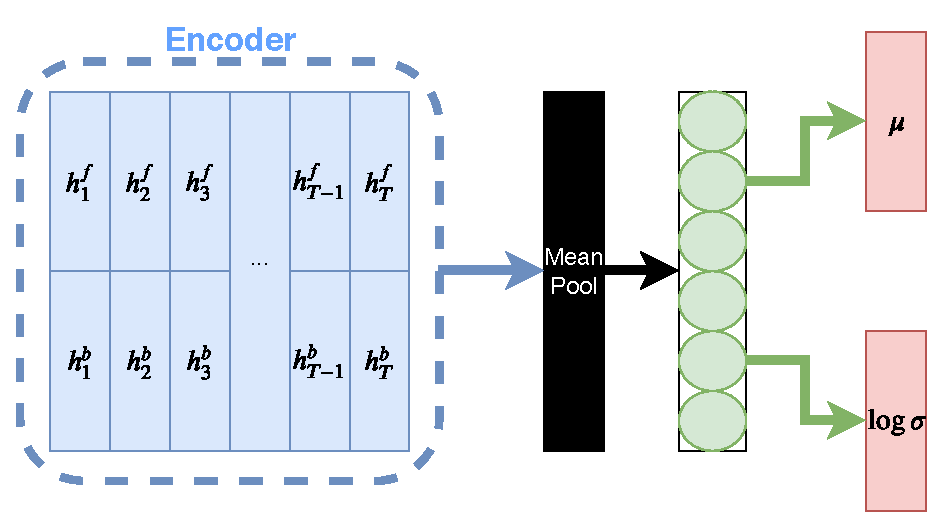
\includegraphics[width=\linewidth]{LatentZEncoding.pdf}
	\caption{General approach to encoding the parameters of the latent variable $Z$ in both models considered in this thesis}
	\label{fig:latentZ}
\end{figure}

